% Options for packages loaded elsewhere
\PassOptionsToPackage{unicode}{hyperref}
\PassOptionsToPackage{hyphens}{url}
\documentclass[
]{article}
\usepackage{xcolor}
\usepackage[margin=1in]{geometry}
\usepackage{amsmath,amssymb}
\setcounter{secnumdepth}{-\maxdimen} % remove section numbering
\usepackage{iftex}
\ifPDFTeX
  \usepackage[T1]{fontenc}
  \usepackage[utf8]{inputenc}
  \usepackage{textcomp} % provide euro and other symbols
\else % if luatex or xetex
  \usepackage{unicode-math} % this also loads fontspec
  \defaultfontfeatures{Scale=MatchLowercase}
  \defaultfontfeatures[\rmfamily]{Ligatures=TeX,Scale=1}
\fi
\usepackage{lmodern}
\ifPDFTeX\else
  % xetex/luatex font selection
\fi
% Use upquote if available, for straight quotes in verbatim environments
\IfFileExists{upquote.sty}{\usepackage{upquote}}{}
\IfFileExists{microtype.sty}{% use microtype if available
  \usepackage[]{microtype}
  \UseMicrotypeSet[protrusion]{basicmath} % disable protrusion for tt fonts
}{}
\makeatletter
\@ifundefined{KOMAClassName}{% if non-KOMA class
  \IfFileExists{parskip.sty}{%
    \usepackage{parskip}
  }{% else
    \setlength{\parindent}{0pt}
    \setlength{\parskip}{6pt plus 2pt minus 1pt}}
}{% if KOMA class
  \KOMAoptions{parskip=half}}
\makeatother
\usepackage{color}
\usepackage{fancyvrb}
\newcommand{\VerbBar}{|}
\newcommand{\VERB}{\Verb[commandchars=\\\{\}]}
\DefineVerbatimEnvironment{Highlighting}{Verbatim}{commandchars=\\\{\}}
% Add ',fontsize=\small' for more characters per line
\usepackage{framed}
\definecolor{shadecolor}{RGB}{248,248,248}
\newenvironment{Shaded}{\begin{snugshade}}{\end{snugshade}}
\newcommand{\AlertTok}[1]{\textcolor[rgb]{0.94,0.16,0.16}{#1}}
\newcommand{\AnnotationTok}[1]{\textcolor[rgb]{0.56,0.35,0.01}{\textbf{\textit{#1}}}}
\newcommand{\AttributeTok}[1]{\textcolor[rgb]{0.13,0.29,0.53}{#1}}
\newcommand{\BaseNTok}[1]{\textcolor[rgb]{0.00,0.00,0.81}{#1}}
\newcommand{\BuiltInTok}[1]{#1}
\newcommand{\CharTok}[1]{\textcolor[rgb]{0.31,0.60,0.02}{#1}}
\newcommand{\CommentTok}[1]{\textcolor[rgb]{0.56,0.35,0.01}{\textit{#1}}}
\newcommand{\CommentVarTok}[1]{\textcolor[rgb]{0.56,0.35,0.01}{\textbf{\textit{#1}}}}
\newcommand{\ConstantTok}[1]{\textcolor[rgb]{0.56,0.35,0.01}{#1}}
\newcommand{\ControlFlowTok}[1]{\textcolor[rgb]{0.13,0.29,0.53}{\textbf{#1}}}
\newcommand{\DataTypeTok}[1]{\textcolor[rgb]{0.13,0.29,0.53}{#1}}
\newcommand{\DecValTok}[1]{\textcolor[rgb]{0.00,0.00,0.81}{#1}}
\newcommand{\DocumentationTok}[1]{\textcolor[rgb]{0.56,0.35,0.01}{\textbf{\textit{#1}}}}
\newcommand{\ErrorTok}[1]{\textcolor[rgb]{0.64,0.00,0.00}{\textbf{#1}}}
\newcommand{\ExtensionTok}[1]{#1}
\newcommand{\FloatTok}[1]{\textcolor[rgb]{0.00,0.00,0.81}{#1}}
\newcommand{\FunctionTok}[1]{\textcolor[rgb]{0.13,0.29,0.53}{\textbf{#1}}}
\newcommand{\ImportTok}[1]{#1}
\newcommand{\InformationTok}[1]{\textcolor[rgb]{0.56,0.35,0.01}{\textbf{\textit{#1}}}}
\newcommand{\KeywordTok}[1]{\textcolor[rgb]{0.13,0.29,0.53}{\textbf{#1}}}
\newcommand{\NormalTok}[1]{#1}
\newcommand{\OperatorTok}[1]{\textcolor[rgb]{0.81,0.36,0.00}{\textbf{#1}}}
\newcommand{\OtherTok}[1]{\textcolor[rgb]{0.56,0.35,0.01}{#1}}
\newcommand{\PreprocessorTok}[1]{\textcolor[rgb]{0.56,0.35,0.01}{\textit{#1}}}
\newcommand{\RegionMarkerTok}[1]{#1}
\newcommand{\SpecialCharTok}[1]{\textcolor[rgb]{0.81,0.36,0.00}{\textbf{#1}}}
\newcommand{\SpecialStringTok}[1]{\textcolor[rgb]{0.31,0.60,0.02}{#1}}
\newcommand{\StringTok}[1]{\textcolor[rgb]{0.31,0.60,0.02}{#1}}
\newcommand{\VariableTok}[1]{\textcolor[rgb]{0.00,0.00,0.00}{#1}}
\newcommand{\VerbatimStringTok}[1]{\textcolor[rgb]{0.31,0.60,0.02}{#1}}
\newcommand{\WarningTok}[1]{\textcolor[rgb]{0.56,0.35,0.01}{\textbf{\textit{#1}}}}
\usepackage{graphicx}
\makeatletter
\newsavebox\pandoc@box
\newcommand*\pandocbounded[1]{% scales image to fit in text height/width
  \sbox\pandoc@box{#1}%
  \Gscale@div\@tempa{\textheight}{\dimexpr\ht\pandoc@box+\dp\pandoc@box\relax}%
  \Gscale@div\@tempb{\linewidth}{\wd\pandoc@box}%
  \ifdim\@tempb\p@<\@tempa\p@\let\@tempa\@tempb\fi% select the smaller of both
  \ifdim\@tempa\p@<\p@\scalebox{\@tempa}{\usebox\pandoc@box}%
  \else\usebox{\pandoc@box}%
  \fi%
}
% Set default figure placement to htbp
\def\fps@figure{htbp}
\makeatother
\setlength{\emergencystretch}{3em} % prevent overfull lines
\providecommand{\tightlist}{%
  \setlength{\itemsep}{0pt}\setlength{\parskip}{0pt}}
\usepackage{bookmark}
\IfFileExists{xurl.sty}{\usepackage{xurl}}{} % add URL line breaks if available
\urlstyle{same}
\hypersetup{
  pdftitle={Assignment-4-Exercise},
  pdfauthor={Vishnun-300665889},
  hidelinks,
  pdfcreator={LaTeX via pandoc}}

\title{Assignment-4-Exercise}
\author{Vishnun-300665889}
\date{2026-09-24}

\begin{document}
\maketitle

Exercise 1

\begin{enumerate}
\def\labelenumi{\arabic{enumi}.}
\tightlist
\item
  Computing of Order Statistic Summary
\end{enumerate}

(H\&F, 1996) had an in-depth look into the nine sample quantile
definition, and their `positive' over other definitions and their
coverage of dealing with distributions. In the end, (H\&F) noted that
the current variation caused confusion, and aimed for standardized
definition across the package, opting for the unbiased variation of
denominator (n-1), adopted by the statistical community. Wicklin's
surmised that despite the many statistical definitions to calculate the
quantile range, by using the same small dataset for their calculation,
the resulting quantile-quantile plots generated differ very slightly.
Depending on the platform used such as R, had a standardized form of
Type 7 as the default form (confirmed using ?quantile)

Personal Opinion: Defintion of Q8, gives a median, unbiased estimator,
while the definition defines the properties are more difficult to
obtain, the resulting use case is more robust and presents a more
accurate result regardless of the distribution, other definitions have
some caveats in that they cannot be used outside the normal distribution
or other types of distributions. Most other definitions that are
distribution-free fall short in a biased estimator. If the goal is for
true accuracy, we require that the order statistic definition do not
fall short of the true population parameter used for estimation.

\begin{enumerate}
\def\labelenumi{\arabic{enumi}.}
\setcounter{enumi}{1}
\tightlist
\item
  Suspicion of IQR is biased, Derive and implement first-order bootstrap
  bias:
\end{enumerate}

\begin{Shaded}
\begin{Highlighting}[]
\NormalTok{lambda\_IQR }\OtherTok{\textless{}{-}} \ControlFlowTok{function}\NormalTok{(x) \{}
\NormalTok{  q }\OtherTok{\textless{}{-}} \FunctionTok{quantile}\NormalTok{(x, }\AttributeTok{probs =} \FunctionTok{c}\NormalTok{(}\FloatTok{0.25}\NormalTok{, }\FloatTok{0.75}\NormalTok{),}
                \AttributeTok{type =} \DecValTok{7}\NormalTok{) }\CommentTok{\#Since type 7 is default}
  \FunctionTok{log}\NormalTok{(}\DecValTok{3}\NormalTok{) }\SpecialCharTok{/}\NormalTok{ q[}\DecValTok{2}\NormalTok{] }\SpecialCharTok{{-}}\NormalTok{ q[}\DecValTok{1}\NormalTok{]}
\NormalTok{\}}
\CommentTok{\#First Order Bootstrap}
\NormalTok{lambda\_hat }\OtherTok{\textless{}{-}} \ControlFlowTok{function}\NormalTok{(x, }\AttributeTok{B =} \DecValTok{200}\NormalTok{) \{}
\NormalTok{  n }\OtherTok{\textless{}{-}} \FunctionTok{length}\NormalTok{(x)}
  
\NormalTok{  lam\_hat }\OtherTok{\textless{}{-}} \FunctionTok{lambda\_IQR}\NormalTok{(x)}
  
\NormalTok{  boot\_estimates }\OtherTok{\textless{}{-}} \FunctionTok{numeric}\NormalTok{(B)}
  \ControlFlowTok{for}\NormalTok{ (b }\ControlFlowTok{in} \DecValTok{1}\SpecialCharTok{:}\NormalTok{B) \{}
\NormalTok{    x\_star }\OtherTok{\textless{}{-}} \FunctionTok{sample}\NormalTok{(x, }\AttributeTok{size =}\NormalTok{ n, }\AttributeTok{replace =} \ConstantTok{TRUE}\NormalTok{)}
\NormalTok{    boot\_estimates[b] }\OtherTok{\textless{}{-}} \FunctionTok{lambda\_IQR}\NormalTok{(x\_star)}
\NormalTok{  \}}
\NormalTok{  bias\_hat }\OtherTok{\textless{}{-}} \FunctionTok{mean}\NormalTok{(boot\_estimates) }\SpecialCharTok{{-}}\NormalTok{ lam\_hat}
  
\NormalTok{  lam\_T }\OtherTok{\textless{}{-}}\NormalTok{ lam\_hat }\SpecialCharTok{{-}}\NormalTok{ bias\_hat}
  
  \FunctionTok{return}\NormalTok{(lam\_T)}
\NormalTok{  \}}
\end{Highlighting}
\end{Shaded}

\begin{Shaded}
\begin{Highlighting}[]
\CommentTok{\#Use Case:}
\FunctionTok{set.seed}\NormalTok{(}\DecValTok{1}\NormalTok{)}
\NormalTok{x }\OtherTok{\textless{}{-}} \FunctionTok{rexp}\NormalTok{(}\AttributeTok{n =} \DecValTok{50}\NormalTok{, }\AttributeTok{rate =} \DecValTok{2}\NormalTok{) }\CommentTok{\#Sample with true lambda = 2}

\FunctionTok{lambda\_IQR}\NormalTok{(x) }\CommentTok{\#Original (Biased) Estimate}
\end{Highlighting}
\end{Shaded}

\begin{verbatim}
##      75% 
## 1.597416
\end{verbatim}

\begin{Shaded}
\begin{Highlighting}[]
\FunctionTok{lambda\_hat}\NormalTok{(x) }\CommentTok{\#Bias Corrected Estimate}
\end{Highlighting}
\end{Shaded}

\begin{verbatim}
##     75% 
## 1.58207
\end{verbatim}

\begin{enumerate}
\def\labelenumi{\arabic{enumi}.}
\setcounter{enumi}{2}
\tightlist
\item
  Monte Carlo Experiment
\end{enumerate}

\begin{Shaded}
\begin{Highlighting}[]
\NormalTok{lambda\_ML }\OtherTok{\textless{}{-}} \ControlFlowTok{function}\NormalTok{(x) \{}
  \DecValTok{1} \SpecialCharTok{/} \FunctionTok{mean}\NormalTok{(x)}
\NormalTok{\}}

\NormalTok{lambda\_tilde }\OtherTok{\textless{}{-}} \ControlFlowTok{function}\NormalTok{(x, }\AttributeTok{B =} \DecValTok{200}\NormalTok{) \{}
\NormalTok{  n }\OtherTok{\textless{}{-}} \FunctionTok{length}\NormalTok{(x)}
  
\NormalTok{  lam\_hat }\OtherTok{\textless{}{-}} \FunctionTok{lambda\_IQR}\NormalTok{(x)}
  
\NormalTok{  boot\_estimates }\OtherTok{\textless{}{-}} \FunctionTok{numeric}\NormalTok{(B)}
  \ControlFlowTok{for}\NormalTok{ (b }\ControlFlowTok{in} \DecValTok{1}\SpecialCharTok{:}\NormalTok{B) \{}
\NormalTok{    x\_star }\OtherTok{\textless{}{-}} \FunctionTok{sample}\NormalTok{(x, }\AttributeTok{size =}\NormalTok{ n, }\AttributeTok{replace =} \ConstantTok{TRUE}\NormalTok{)}
\NormalTok{    boot\_estimates[b] }\OtherTok{\textless{}{-}} \FunctionTok{lambda\_IQR}\NormalTok{(x\_star)}
\NormalTok{  \}}
\NormalTok{  bias\_hat }\OtherTok{\textless{}{-}} \FunctionTok{mean}\NormalTok{(boot\_estimates) }\SpecialCharTok{{-}}\NormalTok{ lam\_hat}
\NormalTok{  lam\_hat }\SpecialCharTok{{-}}\NormalTok{ bias\_hat}

\NormalTok{  \}}

\NormalTok{one\_replication }\OtherTok{\textless{}{-}} \ControlFlowTok{function}\NormalTok{(lambda, n, }\AttributeTok{B =} \DecValTok{200}\NormalTok{) \{}
\NormalTok{  x }\OtherTok{\textless{}{-}} \FunctionTok{rexp}\NormalTok{(n, }\AttributeTok{rate =}\NormalTok{ lambda)}
  
\NormalTok{  est\_ml }\OtherTok{\textless{}{-}} \FunctionTok{lambda\_ML}\NormalTok{(x)}
\NormalTok{  est\_IQR }\OtherTok{\textless{}{-}} \FunctionTok{lambda\_IQR}\NormalTok{(x)}
\NormalTok{  est\_tilde }\OtherTok{\textless{}{-}} \FunctionTok{lambda\_tilde}\NormalTok{(x, }\AttributeTok{B =}\NormalTok{ B)}

  \FunctionTok{c}\NormalTok{(}
    \AttributeTok{ml =}\NormalTok{ (est\_ml }\SpecialCharTok{{-}}\NormalTok{ lambda)}\SpecialCharTok{\^{}}\DecValTok{2}\NormalTok{,}
    \AttributeTok{iqr =}\NormalTok{(est\_IQR }\SpecialCharTok{{-}}\NormalTok{ lambda)}\SpecialCharTok{\^{}}\DecValTok{2}\NormalTok{,}
    \AttributeTok{hat =}\NormalTok{ (est\_tilde }\SpecialCharTok{{-}}\NormalTok{ lambda)}\SpecialCharTok{\^{}}\DecValTok{2}
\NormalTok{  )}
\NormalTok{\}}
\end{Highlighting}
\end{Shaded}

\begin{Shaded}
\begin{Highlighting}[]
\NormalTok{mc\_converg }\OtherTok{\textless{}{-}} \ControlFlowTok{function}\NormalTok{(lambda, n , R\_max, }\AttributeTok{B =} \DecValTok{200}\NormalTok{) \{}
\NormalTok{  sq\_errors }\OtherTok{\textless{}{-}} \FunctionTok{matrix}\NormalTok{(}\ConstantTok{NA}\NormalTok{, }\AttributeTok{nrow =}\NormalTok{ R\_max, }\AttributeTok{ncol =} \DecValTok{3}\NormalTok{)}
  \FunctionTok{colnames}\NormalTok{(sq\_errors) }\OtherTok{\textless{}{-}} \FunctionTok{c}\NormalTok{(}\StringTok{"ML"}\NormalTok{, }\StringTok{"IQR"}\NormalTok{, }\StringTok{"Tilde"}\NormalTok{)}
  
  \ControlFlowTok{for}\NormalTok{ (r }\ControlFlowTok{in} \DecValTok{1}\SpecialCharTok{:}\NormalTok{R\_max) \{}
\NormalTok{    sq\_errors[r, ] }\OtherTok{\textless{}{-}} \FunctionTok{one\_replication}\NormalTok{(lambda, n, }\AttributeTok{B =}\NormalTok{ B)}
\NormalTok{  \}}

\NormalTok{fall\_MSE }\OtherTok{\textless{}{-}} \FunctionTok{apply}\NormalTok{(sq\_errors, }\DecValTok{2}\NormalTok{, }\ControlFlowTok{function}\NormalTok{(col) }\FunctionTok{cumsum}\NormalTok{(col) }\SpecialCharTok{/} \FunctionTok{seq\_along}\NormalTok{(col))}

\NormalTok{foll\_se }\OtherTok{\textless{}{-}} \FunctionTok{matrix}\NormalTok{(}\ConstantTok{NA}\NormalTok{, }\AttributeTok{nrow =}\NormalTok{ R\_max, }\AttributeTok{ncol =} \DecValTok{3}\NormalTok{)}
\FunctionTok{colnames}\NormalTok{(fall\_MSE) }\OtherTok{\textless{}{-}} \FunctionTok{c}\NormalTok{(}\StringTok{"ML"}\NormalTok{, }\StringTok{"IQR"}\NormalTok{, }\StringTok{"Tilde"}\NormalTok{)}

\ControlFlowTok{for}\NormalTok{(j }\ControlFlowTok{in} \DecValTok{1}\SpecialCharTok{:}\DecValTok{3}\NormalTok{) \{}
  \ControlFlowTok{for}\NormalTok{(r }\ControlFlowTok{in} \DecValTok{2}\SpecialCharTok{:}\NormalTok{R\_max) \{}
\NormalTok{    v\_r }\OtherTok{\textless{}{-}} \FunctionTok{var}\NormalTok{(sq\_errors[}\DecValTok{1}\SpecialCharTok{:}\NormalTok{r, j])}
\NormalTok{    foll\_se[r, j] }\OtherTok{\textless{}{-}} \FunctionTok{sqrt}\NormalTok{(v\_r }\SpecialCharTok{/}\NormalTok{ r)}
\NormalTok{  \}}
\NormalTok{\} }

\FunctionTok{list}\NormalTok{(}\AttributeTok{sq\_errors =}\NormalTok{ sq\_errors, }\AttributeTok{fall\_MSE =}\NormalTok{ fall\_MSE, }\AttributeTok{foll\_se =}\NormalTok{ foll\_se)}
\NormalTok{\}}
\end{Highlighting}
\end{Shaded}

\begin{Shaded}
\begin{Highlighting}[]
\FunctionTok{set.seed}\NormalTok{(}\DecValTok{42}\NormalTok{)}

\NormalTok{result }\OtherTok{\textless{}{-}} \FunctionTok{mc\_converg}\NormalTok{(}\AttributeTok{lambda =} \DecValTok{1}\NormalTok{, }\AttributeTok{n =} \DecValTok{5}\NormalTok{, }\AttributeTok{R\_max =} \DecValTok{2000}\NormalTok{, }\AttributeTok{B =} \DecValTok{200}\NormalTok{)}
\end{Highlighting}
\end{Shaded}

Visual of Convergence Check simulation methods

\begin{Shaded}
\begin{Highlighting}[]
\FunctionTok{matplot}\NormalTok{(result}\SpecialCharTok{$}\NormalTok{fall\_MSE, }\AttributeTok{type =} \StringTok{"l"}\NormalTok{, }\AttributeTok{lty =} \DecValTok{1}\NormalTok{, }\AttributeTok{lwd =} \DecValTok{2}\NormalTok{,}
        \AttributeTok{col =} \FunctionTok{c}\NormalTok{(}\StringTok{"blue"}\NormalTok{, }\StringTok{"red"}\NormalTok{, }\StringTok{"darkgreen"}\NormalTok{),}
        \AttributeTok{xlab =} \StringTok{"Number of replications (R)"}\NormalTok{, }\AttributeTok{ylab =} \StringTok{"MSE estimate"}\NormalTok{,}
        \AttributeTok{main =} \StringTok{"Convergence of MSE Estimate"}\NormalTok{)}
\FunctionTok{legend}\NormalTok{(}\StringTok{"topright"}\NormalTok{, }\AttributeTok{legend =} \FunctionTok{c}\NormalTok{(}\StringTok{"ML"}\NormalTok{, }\StringTok{"IQR"}\NormalTok{, }\StringTok{"Tilde"}\NormalTok{),}
       \AttributeTok{col =} \FunctionTok{c}\NormalTok{(}\StringTok{"blue"}\NormalTok{, }\StringTok{"red"}\NormalTok{, }\StringTok{"darkgreen"}\NormalTok{), }\AttributeTok{lty =} \DecValTok{1}\NormalTok{, }\AttributeTok{lwd =} \DecValTok{2}\NormalTok{)}
\end{Highlighting}
\end{Shaded}

\pandocbounded{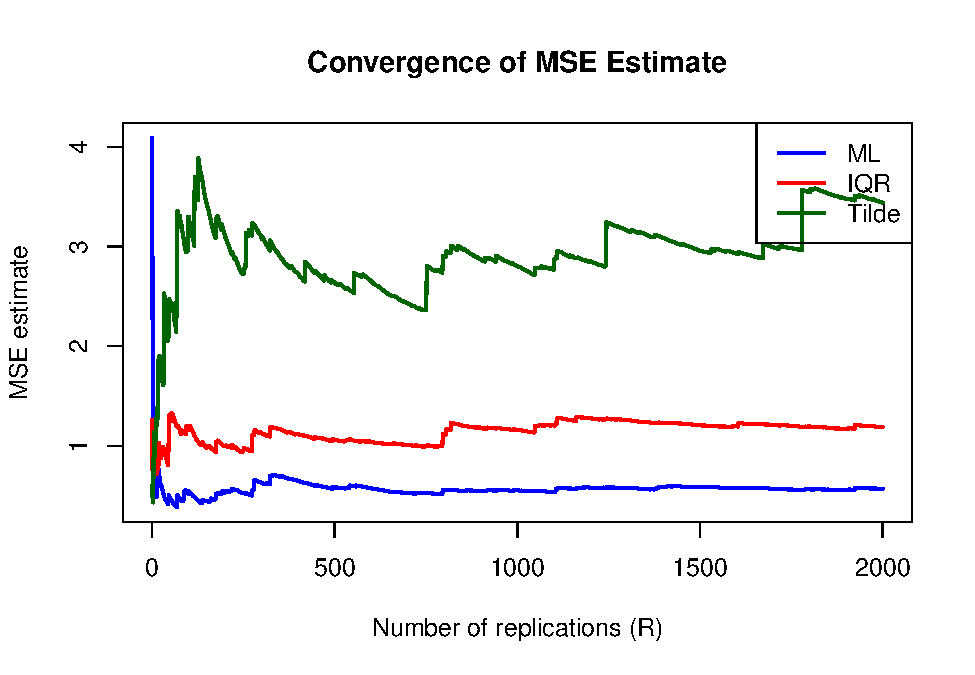
\includegraphics[keepaspectratio]{Assignment-4-Exercise_files/figure-latex/unnamed-chunk-6-1.pdf}}
Monte Carlo SE

\begin{Shaded}
\begin{Highlighting}[]
\FunctionTok{matplot}\NormalTok{(result}\SpecialCharTok{$}\NormalTok{foll\_se,  }\AttributeTok{type =} \StringTok{"l"}\NormalTok{, }\AttributeTok{lty =} \DecValTok{1}\NormalTok{, }\AttributeTok{lwd =} \DecValTok{2}\NormalTok{,}
        \AttributeTok{col =} \FunctionTok{c}\NormalTok{(}\StringTok{"blue"}\NormalTok{, }\StringTok{"red"}\NormalTok{, }\StringTok{"darkgreen"}\NormalTok{),}
        \AttributeTok{xlab =} \StringTok{"Number of replications (R)"}\NormalTok{, }\AttributeTok{ylab =} \StringTok{"Monte Carlo SE of MSE estimate"}\NormalTok{,}
        \AttributeTok{main =} \StringTok{"Monte Carlo SE vs R"}\NormalTok{)}
\FunctionTok{legend}\NormalTok{(}\StringTok{"topright"}\NormalTok{, }\AttributeTok{legend =} \FunctionTok{c}\NormalTok{(}\StringTok{"ML"}\NormalTok{, }\StringTok{"IQR"}\NormalTok{, }\StringTok{"Tilde"}\NormalTok{),}
       \AttributeTok{col =} \FunctionTok{c}\NormalTok{(}\StringTok{"blue"}\NormalTok{, }\StringTok{"red"}\NormalTok{, }\StringTok{"darkgreen"}\NormalTok{), }\AttributeTok{lty =} \DecValTok{1}\NormalTok{, }\AttributeTok{lwd =} \DecValTok{2}\NormalTok{)}
\end{Highlighting}
\end{Shaded}

\pandocbounded{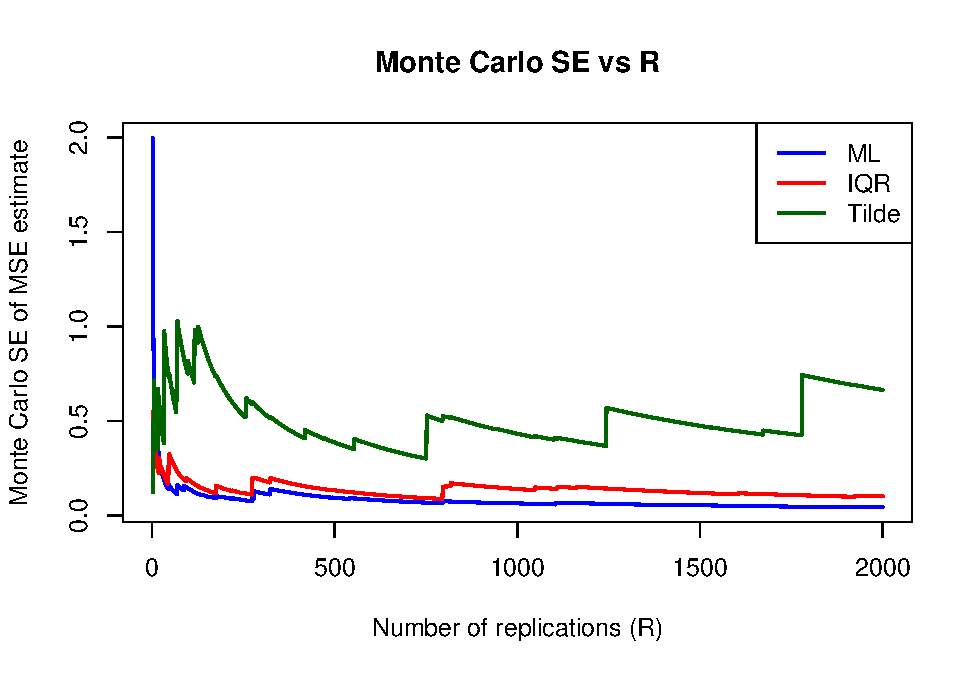
\includegraphics[keepaspectratio]{Assignment-4-Exercise_files/figure-latex/unnamed-chunk-7-1.pdf}}

Full Experiment

\begin{Shaded}
\begin{Highlighting}[]
\NormalTok{lambda\_grid }\OtherTok{\textless{}{-}} \FunctionTok{c}\NormalTok{(}\FloatTok{0.1}\NormalTok{, }\DecValTok{1}\NormalTok{, }\DecValTok{10}\NormalTok{)}
\NormalTok{n\_grid }\OtherTok{\textless{}{-}} \FunctionTok{c}\NormalTok{(}\DecValTok{5}\NormalTok{, }\DecValTok{30}\NormalTok{, }\DecValTok{100}\NormalTok{)}
\NormalTok{R\_grid }\OtherTok{\textless{}{-}} \FunctionTok{c}\NormalTok{(}\StringTok{\textasciigrave{}}\AttributeTok{5}\StringTok{\textasciigrave{}} \OtherTok{=} \DecValTok{5000}\NormalTok{, }\StringTok{\textasciigrave{}}\AttributeTok{30}\StringTok{\textasciigrave{}} \OtherTok{=} \DecValTok{2000}\NormalTok{, }\StringTok{\textasciigrave{}}\AttributeTok{100}\StringTok{\textasciigrave{}} \OtherTok{=} \DecValTok{1000}\NormalTok{)}

\NormalTok{results }\OtherTok{\textless{}{-}} \FunctionTok{data.frame}\NormalTok{()}

\FunctionTok{set.seed}\NormalTok{(}\DecValTok{42}\NormalTok{)}

\ControlFlowTok{for}\NormalTok{ (lambda }\ControlFlowTok{in}\NormalTok{ lambda\_grid) \{}
 \ControlFlowTok{for}\NormalTok{ (n }\ControlFlowTok{in}\NormalTok{ n\_grid) \{}
\NormalTok{   R }\OtherTok{\textless{}{-}}\NormalTok{ R\_grid[}\FunctionTok{as.character}\NormalTok{(n)]}
   
\NormalTok{   sq\_errors }\OtherTok{\textless{}{-}} \FunctionTok{matrix}\NormalTok{(}\ConstantTok{NA}\NormalTok{, }\AttributeTok{nrow =}\NormalTok{ R, }\AttributeTok{ncol =} \DecValTok{3}\NormalTok{)}
   \FunctionTok{colnames}\NormalTok{(sq\_errors) }\OtherTok{\textless{}{-}} \FunctionTok{c}\NormalTok{(}\StringTok{"ML"}\NormalTok{, }\StringTok{"IQR"}\NormalTok{, }\StringTok{"Tilde"}\NormalTok{)}
   
   \ControlFlowTok{for}\NormalTok{ (r }\ControlFlowTok{in} \DecValTok{1}\SpecialCharTok{:}\NormalTok{R) \{}
\NormalTok{     sq\_errors[r, ] }\OtherTok{\textless{}{-}} \FunctionTok{one\_replication}\NormalTok{(lambda, n, }\AttributeTok{B =} \DecValTok{200}\NormalTok{)}
\NormalTok{   \}}
\NormalTok{   mse }\OtherTok{\textless{}{-}} \FunctionTok{colMeans}\NormalTok{(sq\_errors)}
   
\NormalTok{   results }\OtherTok{\textless{}{-}} \FunctionTok{rbind}\NormalTok{(results, }\FunctionTok{data.frame}\NormalTok{(}
     \AttributeTok{lambda =}\NormalTok{ lambda,}
     \AttributeTok{n =}\NormalTok{ n,}
     \AttributeTok{R =}\NormalTok{ R,}
     \AttributeTok{MSE\_ML =}\NormalTok{ mse[}\StringTok{"ML"}\NormalTok{],}
     \AttributeTok{MSE\_IQR =}\NormalTok{ mse[}\StringTok{"IQR"}\NormalTok{],}
     \AttributeTok{MSE\_Tilde =}\NormalTok{ mse[}\StringTok{"Tilde"}\NormalTok{]}
\NormalTok{   ))}
\NormalTok{ \} }
\NormalTok{\}}

\FunctionTok{rownames}\NormalTok{(results) }\OtherTok{\textless{}{-}} \ConstantTok{NULL}
\NormalTok{clean\_results }\OtherTok{\textless{}{-}}\NormalTok{ results}
\NormalTok{clean\_results[ ,}\DecValTok{4}\SpecialCharTok{:}\DecValTok{6}\NormalTok{] }\OtherTok{\textless{}{-}} \FunctionTok{round}\NormalTok{(clean\_results[ ,}\DecValTok{4}\SpecialCharTok{:}\DecValTok{6}\NormalTok{], }\DecValTok{4}\NormalTok{)}
\FunctionTok{print}\NormalTok{(clean\_results)}
\end{Highlighting}
\end{Shaded}

\begin{verbatim}
##   lambda   n    R  MSE_ML MSE_IQR MSE_Tilde
## 1    0.1   5 5000  0.0060 30.5247   32.4515
## 2    0.1  30 2000  0.0004 11.3234   10.6321
## 3    0.1 100 1000  0.0001  9.4610    9.2450
## 4    1.0   5 5000  0.6071  1.2056   13.1227
## 5    1.0  30 2000  0.0394  0.2949    0.3197
## 6    1.0 100 1000  0.0105  0.2567    0.2633
## 7   10.0   5 5000 50.7400 63.8940  917.6861
## 8   10.0  30 2000  3.9489  6.4778    8.5829
## 9   10.0 100 1000  1.0245  5.0457    5.6132
\end{verbatim}

Plot Convergence Report: ML (Blue) settling the fastest and lowest, and
is the `best' estimator when the model is correctly specified, outcome
has both low bias and low variance IQR (Red) slightly higher than ML,
only taking slightly longer, relatively just as smooth. Tilde (Green) is
the highest, still have spikes even with R = 500 replications. It didn't
converge properly.

Monte Carlo Tilde (Green) with large standard error is still large, and
wasn't flatten by R = 500, while ML and IQR have stablised well much
sooner.

Why the Lambda\^{}Tilde (Green) still perform badly in both iterations,
the difference in quartile 3/4 and quartile 1/4 can be small by chance.
This makes the \(\lambda_{IQR}\) = ln 3 / \(q_{3/4(X)}\) −
\(𝑞_{1/4(X)}\) blow up. This bootstrap correction than compounds this,
resampling from the same small, already unstable sample. Son on
unfavorable replications, the correction can massively overshoot,
producing occasional huge squared errors as shown as sharp spikes within
the plots.

Therefore, increasing the R in theory should help the SE and potentially
flatten the lines within the plot. For n = 5, lambda should hold the
instability.

However, despite increasing the R = 2000, no meaningful changes is
observed, and no smoothing effect. At n = 5, the Monte Carlo estimate of
MSE for \(\lambda\) tilde did not stablise at R = 2000, observing
extreme outlying values consistent with a heavy tailed sampling
distribution for this estimator in small samples.

Final Report: MSE grows with n growth, at n = 100, MSE\_ML at
\(\lambda = 0,1, 1, 10\) is roughly 0.0001, 0.0105, and 1.0245, all
three values matching the MLE asymptotic variance of \(\lambda^{hat}\)
is \(\lambda^2 / n\). This match proves simulation is behaving correctly
and ML performing uniformly the best.

The \(\lambda^{tilde}\) vs \(\lambda^{hat}\) comparison, the bootstrap
bias correction did not improve on the plain IQR estimator in this
experiment. At n increases, the value of MSE performance improves,
smaller n, performs horribly particularly paired with large \(\lambda\)

\begin{enumerate}
\def\labelenumi{\arabic{enumi}.}
\setcounter{enumi}{1}
\tightlist
\item
\end{enumerate}

\begin{Shaded}
\begin{Highlighting}[]
\FunctionTok{library}\NormalTok{(fpp2)}
\end{Highlighting}
\end{Shaded}

\begin{verbatim}
## Warning: package 'fpp2' was built under R version 4.5.2
\end{verbatim}

\begin{verbatim}
## -- Attaching packages -------------------------------------------- fpp2 2.5.1 --
\end{verbatim}

\begin{verbatim}
## v ggplot2   4.0.3     v fma       2.5  
## v forecast  9.0.1     v expsmooth 2.3
\end{verbatim}

\begin{verbatim}
## Warning: package 'ggplot2' was built under R version 4.5.2
\end{verbatim}

\begin{verbatim}
## Warning: package 'forecast' was built under R version 4.5.2
\end{verbatim}

\begin{verbatim}
## 
\end{verbatim}

\begin{Shaded}
\begin{Highlighting}[]
\FunctionTok{data}\NormalTok{(}\StringTok{"ausbeer"}\NormalTok{)}
\FunctionTok{head}\NormalTok{(ausbeer)}
\end{Highlighting}
\end{Shaded}

\begin{verbatim}
##      Qtr1 Qtr2 Qtr3 Qtr4
## 1956  284  213  227  308
## 1957  262  228
\end{verbatim}

\begin{enumerate}
\def\labelenumi{\arabic{enumi}.}
\tightlist
\item
\end{enumerate}

\begin{Shaded}
\begin{Highlighting}[]
\FunctionTok{autoplot}\NormalTok{(ausbeer) }\SpecialCharTok{+} 
  \FunctionTok{ggtitle}\NormalTok{(}\StringTok{"Quarterly Australian Beer Production"}\NormalTok{) }\SpecialCharTok{+}
  \FunctionTok{xlab}\NormalTok{(}\StringTok{"Year"}\NormalTok{) }\SpecialCharTok{+} \FunctionTok{ylab}\NormalTok{(}\StringTok{"Megalitres"}\NormalTok{)}
\end{Highlighting}
\end{Shaded}

\pandocbounded{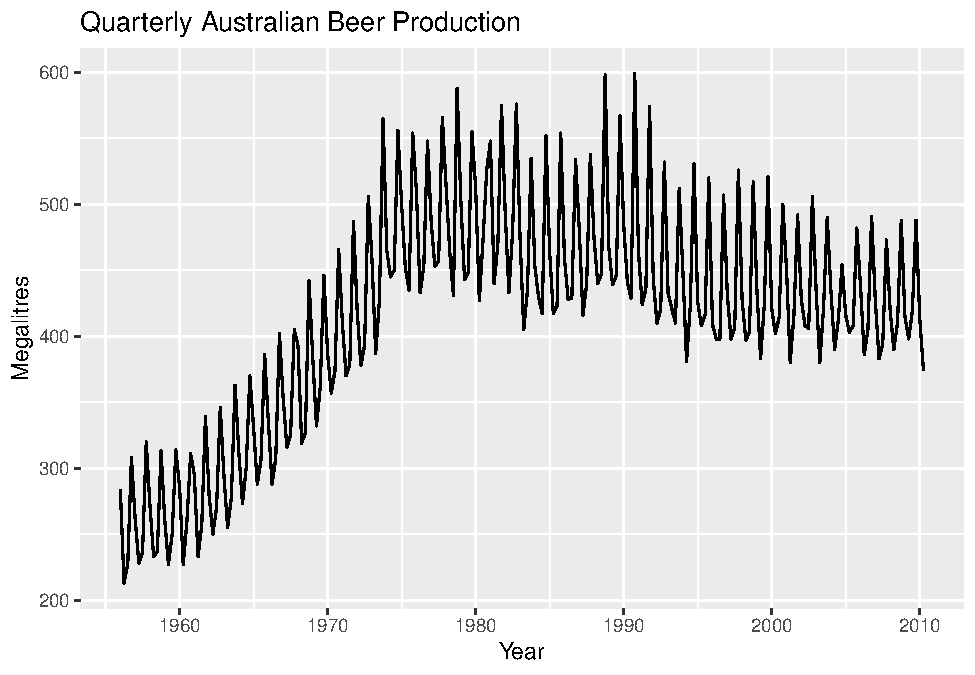
\includegraphics[keepaspectratio]{Assignment-4-Exercise_files/figure-latex/unnamed-chunk-11-1.pdf}}
Interpretation: Frequency based on observation is ``Quarterly'' beer
production, hence for our time series, Frequency observation per year is
four, and each one unit ``peak'' along the (X-axis) are individual years
that contain one full up and down cycle made roughly of 4 data points,
one rise, one peak, one fall, and one lowest minimum point. Each pattern
change of the individual ``peak'' show us that four point per year.

\begin{enumerate}
\def\labelenumi{\arabic{enumi}.}
\setcounter{enumi}{1}
\item
  We can note the trend of beer production increases significantly and
  follow an upward trend from 1960s to 1990s, followed by gradual
  decline from the earl 1990s to 2010s.
\item
  I can comment on the seasonal changes of the individual years, this
  consistent peak point and low points tells us there is significant
  contribution from seasonal changes that affects beer production. This
  consistency aligns with high quarters and low quarters each year that
  can be explained by seasonal demands such as summer vs winter for beer
  production. The size of the seasonal changes is not always constant
  over time, the gap between peak and lowest production grows from 1960s
  to the 1980s, appearing around the largest around 1980s to 1990s, and
  shortening again around 2010s.
\item
  Variability refer to the seasonal fluctuation gap of the peak and the
  lowest point here, the levels seen here locally grow and shrink as the
  time progresses hence variability is not constant also noting the
  growth from 1960s and shrinking somewhat later around 2010s. A pattern
  consistent with variance that scales with the mean. This is exactly
  the kind of situation a log transformation is appropriate, and its
  application would help stabilise the seasonal swings across the
  series.
\item
  Based on observation, there seems to be two points in time that beer
  production that reaches the highest level of around 600 megalitres in
  1988 and 1991 respectively, in comparison to the peaks before and
  after, which sits around 540 to 580 megalitres, breaking an otherwise
  smooth, gradual progression of peak heights that was seen in seasonal
  patterns. Afterward, there is a steady decline in production, and this
  suggest a long term trend was coincidential in timing, events that is
  worth flagging, perhaps reasoning may be due to anomalies in
  production or consumer demand.
\item
\end{enumerate}

\begin{Shaded}
\begin{Highlighting}[]
\FunctionTok{ggseasonplot}\NormalTok{(ausbeer, }\AttributeTok{polar =} \ConstantTok{TRUE}\NormalTok{) }\SpecialCharTok{+}
  \FunctionTok{ylab}\NormalTok{(}\StringTok{"Megalitres"}\NormalTok{) }\SpecialCharTok{+}
  \FunctionTok{ggtitle}\NormalTok{(}\StringTok{"Polar Seasonal Plot of Quarterly Beer Production in Australia"}\NormalTok{)}
\end{Highlighting}
\end{Shaded}

\pandocbounded{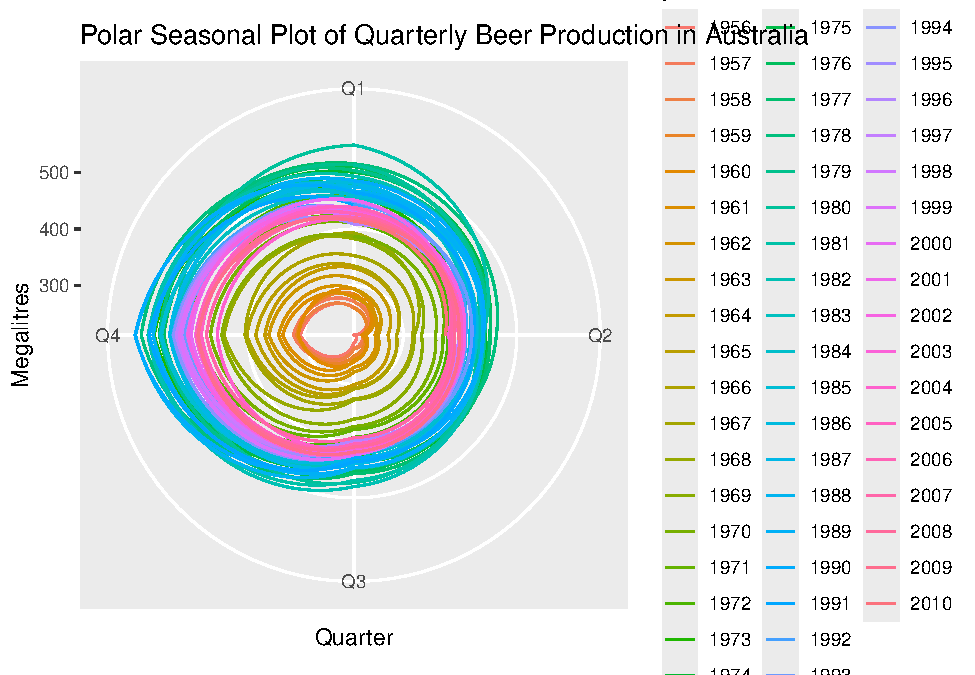
\includegraphics[keepaspectratio]{Assignment-4-Exercise_files/figure-latex/unnamed-chunk-12-1.pdf}}

\begin{Shaded}
\begin{Highlighting}[]
\FunctionTok{ggseasonplot}\NormalTok{(ausbeer, }\AttributeTok{year.labels =} \ConstantTok{TRUE}\NormalTok{, }\AttributeTok{year.labels.left =} \ConstantTok{TRUE}\NormalTok{) }\SpecialCharTok{+}
  \FunctionTok{ylab}\NormalTok{(}\StringTok{"Megalitres"}\NormalTok{) }\SpecialCharTok{+}
  \FunctionTok{ggtitle}\NormalTok{(}\StringTok{"Seasonal Plot of Beer Production in Australia"}\NormalTok{)}
\end{Highlighting}
\end{Shaded}

\pandocbounded{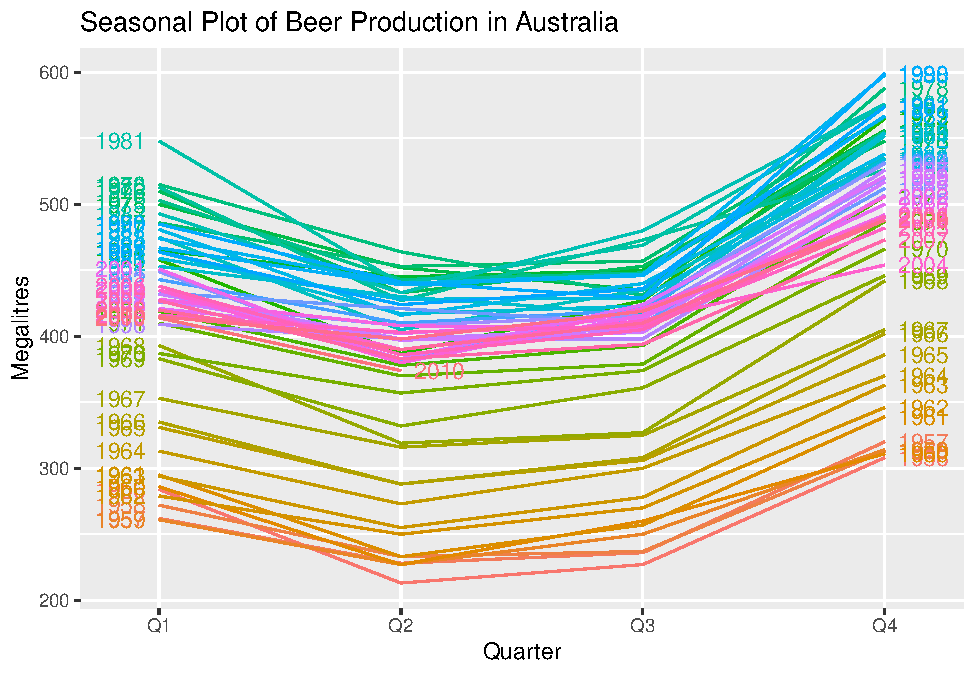
\includegraphics[keepaspectratio]{Assignment-4-Exercise_files/figure-latex/unnamed-chunk-13-1.pdf}}
Based on observation of the two seasonal plots above, we can see a
clearer picture of seasonal patterns itself, each year follow a similar
basic shape, high in Q1, lowest point in Q2, rising in Q3, peaking in Q4
and these patterns repeat consistently over the years. This advantage in
over the original time series plot, where seasonal fluctuation and long
term trend are combined into a single line, making it harder to isolate
the shape of the season. In the seasonal pot, the trend show as a
vertical stack of the colored lines by year, highest line following
1980s to 1990s, while earlier stacks in 1950s to 1960s and 2010s sit
lower. This matches the patterns seen in the time series plot, but this
plot separates the seasonal shape rather than mixing it.

\begin{enumerate}
\def\labelenumi{\arabic{enumi}.}
\setcounter{enumi}{6}
\tightlist
\item
\end{enumerate}

\begin{Shaded}
\begin{Highlighting}[]
\FunctionTok{ggsubseriesplot}\NormalTok{(ausbeer) }\SpecialCharTok{+} 
  \FunctionTok{ylab}\NormalTok{(}\StringTok{"Megalitres"}\NormalTok{) }\SpecialCharTok{+} 
  \FunctionTok{ggtitle}\NormalTok{(}\StringTok{"Seasonal Subseries plot: Beer Production in Australia"}\NormalTok{)}
\end{Highlighting}
\end{Shaded}

\pandocbounded{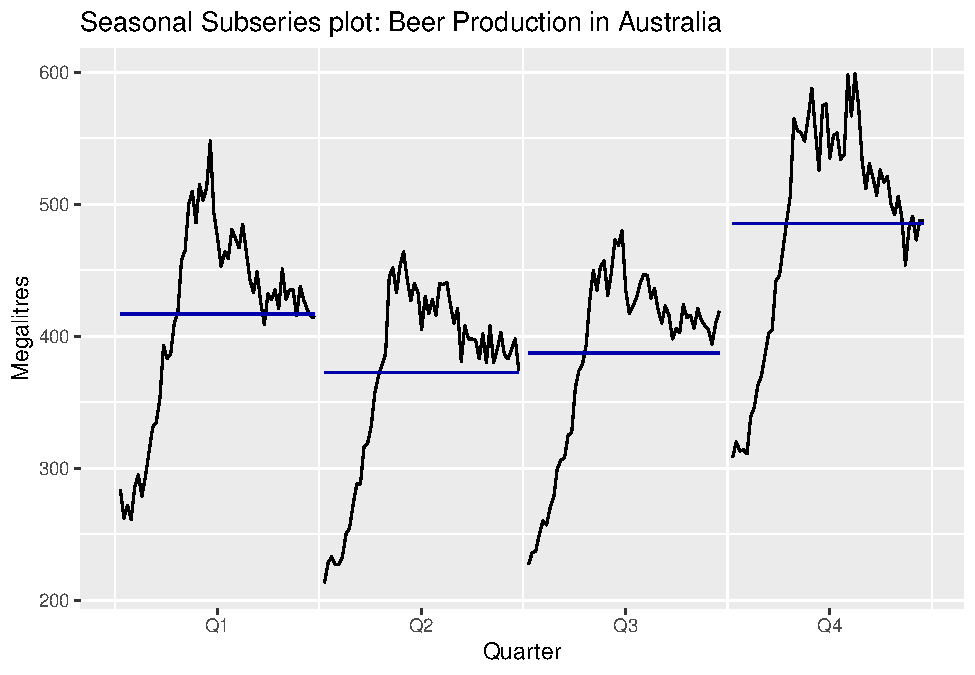
\includegraphics[keepaspectratio]{Assignment-4-Exercise_files/figure-latex/unnamed-chunk-14-1.pdf}}
Based on observation, we can see the means for each quarter, showing an
underlying pattern in seasonal changes and shown more clearly. Q1 as
second highest following the previous quarter, Q2 has the lowest mean,
Q3 is rising again, and Q4 has the highest mean in production. this
consistency can be seen with the seasonal plot and and following the
trend of the time series plot. Looking at each quarter's panel, the
level is not perfectly stable over time, each panel's line rise and
falls following the same long term trend seen in the over series,
climbing from 1950s to 1960s, peaking around 1980s to 1990s, and
declining toward 2010s, with the largest deviations from the quarter's
mean occurring during that peak time. So in terms of relative ordering
of the quarters Q4 being highest, Q2 being lowest is seen consistently
throughout the series plotting. The level of production within each
quarter is not stable, and is similar to the broader trend and changing
variability identified earlier.

\begin{enumerate}
\def\labelenumi{\arabic{enumi}.}
\setcounter{enumi}{7}
\tightlist
\item
\end{enumerate}

\begin{Shaded}
\begin{Highlighting}[]
\FunctionTok{library}\NormalTok{(ggplot2) }
\FunctionTok{library}\NormalTok{(gridExtra)}

\NormalTok{plot1 }\OtherTok{\textless{}{-}} \FunctionTok{autoplot}\NormalTok{(ausbeer) }\SpecialCharTok{+} 
  \FunctionTok{labs}\NormalTok{(}\AttributeTok{title =} \StringTok{"Original Series"}\NormalTok{, }\AttributeTok{y =} \StringTok{"Megalitres"}\NormalTok{)}

\NormalTok{plot2}\OtherTok{\textless{}{-}} \FunctionTok{autoplot}\NormalTok{(}\FunctionTok{log}\NormalTok{(ausbeer)) }\SpecialCharTok{+}
  \FunctionTok{labs}\NormalTok{(}\AttributeTok{title =} \StringTok{"Log{-}transformed series"}\NormalTok{, }\AttributeTok{y =} \StringTok{"log(Megalitres)"}\NormalTok{)}

\FunctionTok{grid.arrange}\NormalTok{(plot1, plot2, }\AttributeTok{ncol =} \DecValTok{1}\NormalTok{)}
\end{Highlighting}
\end{Shaded}

\pandocbounded{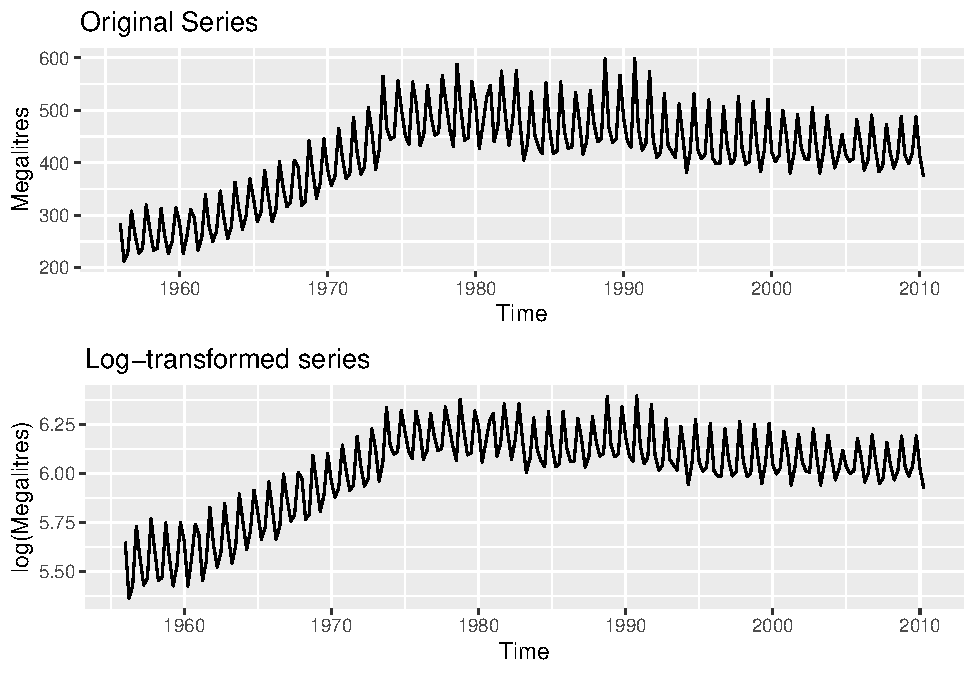
\includegraphics[keepaspectratio]{Assignment-4-Exercise_files/figure-latex/unnamed-chunk-15-1.pdf}}
Detrending is worth doing due to the evidence seen in time series plot
and the seasonal plot color stacking. The time series show a clear
non-stationary trend, rising sharply during 1950s to 1990s, then
declining in 2010s. The season plot backs this with clearer stacking
visuals, each line by year. The time series models assume a constant
mean level roughly. This series doesn't have one, so detrending is
needed before modelling.

Transforming is also worth doing due to our earlier evidence in
variability, the seasonal spiking isn't constant, its small in 1960s,
growing towards 1990s, and declining again later. This growth swinging
tracks the growth in the series overall level over the same period. The
sub series plot making this visible during each quarter's panel, showing
the deviation from the horizontal line. This spike swinging increasing
alongside the level is where a log transformation is commonly used and
help with stabilisation of the variance, making it more constant
regardless of the series level.

Based on the observation of the two plots above, we can see the swing in
the original series, the same pattern spiking in the 600 megalitres
being produced, the growth from 1960s to 1990s and slow decline to
2010s.

However the log series swing in the 1980s to 1990s spike is relatively
smaller to the original. This change in log transformation while not the
most dramatic in change, were worth being investigated, and proved a
slight improvement in stablisation of the variance, while not fully
getting rid of the changing spread on its own.

\end{document}
